The DLR Institute for the Protection of Maritime Infrastructures is consistently working on systems to improve the situational awareness of maritime infrastructures. Part of those awareness systems is the near real-time tracking of vessels and the detection of abnormal ship behaviour. Such anomalies can potentially range from unusual trajectories, entry into restricted zones, speeding and intentional AIS on-off switching to actual collisions or pirate attacks.
\par
Although all of those anomaly types are important, this thesis specifically focuses on the detection of abnormal vessel trajectories.  The assumption that can be made here is that by abstracting ship behaviour to the raw movement output while also taking into account different non-kinematic information, it is possible to implicitly detect multiple anomaly types without labeling them explicitly. 
\par
The main approach to this problem is to train a model that is capable of predicting future \anf{normal} trajectories to then compare those to the real paths. If the difference between the two trajectories exceeds a certain threshold it gets labeled anomalous. Previous work at the institute regarding this topic involved the usage of sequential models like LSTMs. The downside of those network architectures is the requirement of a predefined-length frame of timestamps as input that eventually leads to a prediction of a fixed output window. An end-to-end path prediction has low performance due to the observed phenomena that sequentially take a predicted output as input sequence leads to significant error accumulation as displayed in figure \ref{fig:lstm}. 
\begin{figure}[H]
    \centering
    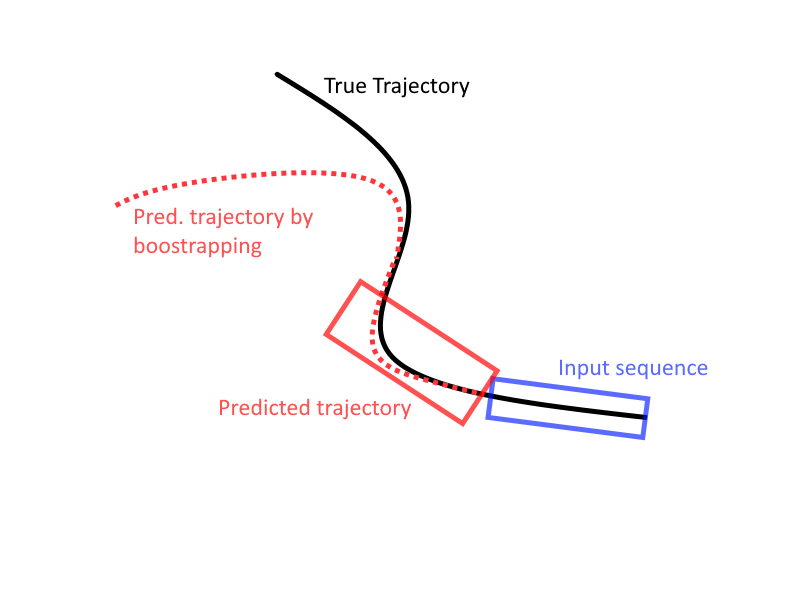
\includegraphics[width=0.75\textwidth]{images/LSTM_trajectory_window_example.png}
    \caption{Illustration of the accumulated prediction error by bootstrapping input sequences for an LSTM}
    \label{fig:lstm}
\end{figure}
With the rise of deep reinforcement learning and its successful application in fields like robot control and autonomous system (\cite{s18092905, zare2021continuous, 9195789, martinsen2018curved}), the question comes to mind if this task can be formulated as a reinforcement learning problem as well. The idea behind using reinforcement learning is that training an agent to control an unmanned vessel results in a policy that learns end-to-end trajectories to get to a predefined destination. By replacing the simulated real-world environment with samples from normal vessel trajectories and tweaking the reward function, the assumption is that the agent learns to mimic normal vessel behaviour to eventually predict end-to-end trajectories.
\par
To give an example of what the agent should eventually learn, we illustrate two density maps of vessel trajectories generated by \cite{martinetraffic} for the year 2020:
\begin{figure}[H]
    \centering
    \begin{minipage}{.47\textwidth}
      \centering
      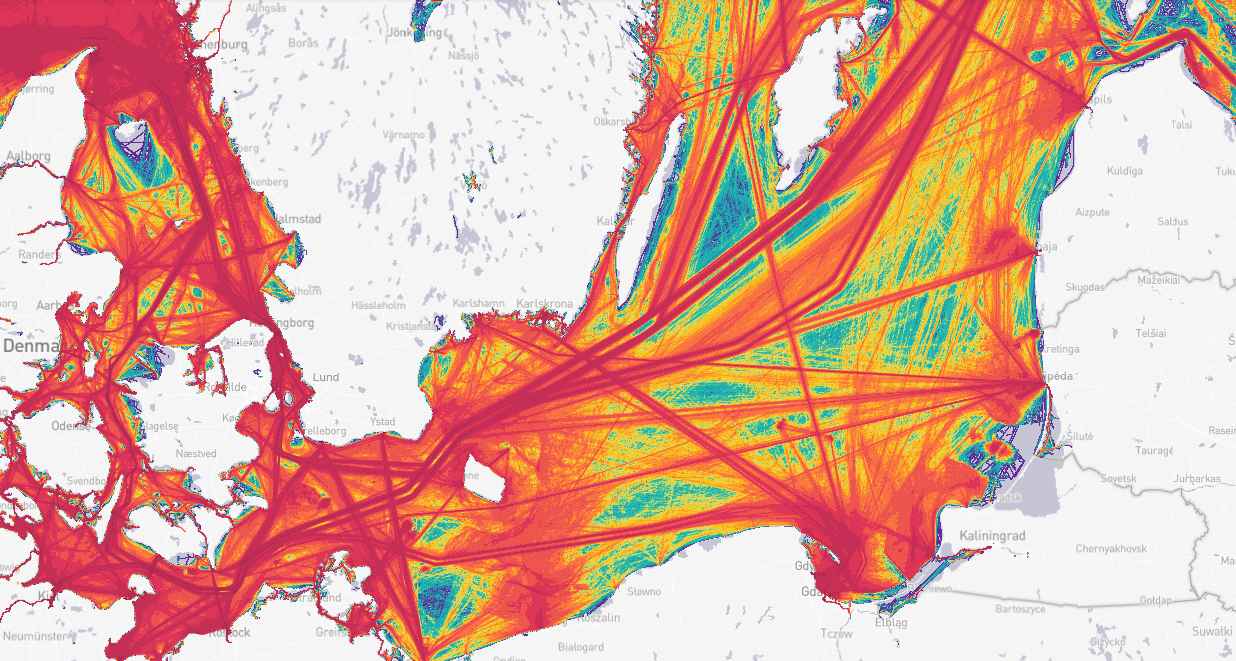
\includegraphics[width=\textwidth]{images/balticsea_density_routes.PNG}
      \captionof{figure}{Density map of vessel trajectories in the Baltic Sea}
      \label{fig:baltic}
    \end{minipage}
    \hspace{.05\textwidth}%
    \begin{minipage}{.47\textwidth}
        \centering
        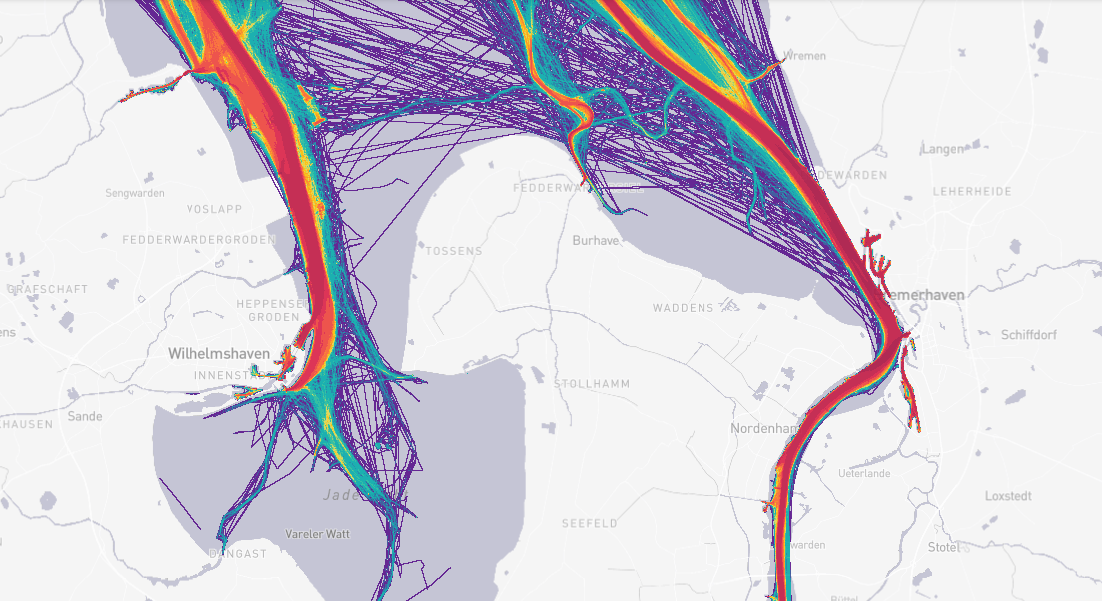
\includegraphics[width=\textwidth]{images/bhv_jadebusen_density_routes.PNG}
        \captionof{figure}{Density map of vessels near Bremerhaven and the Jadebusen}
        \label{fig:jadebusen}
      \end{minipage}
\end{figure}
Looking at figure \ref{fig:baltic}, we can discover the international shipping routes by following the red lines which indicate a high volume of vessel traffic. Furthermore, we notice certain points where the majority of ships choose to somewhat suddenly change their heading. It is up to the agent to learn exactly those specific patterns as in break points, entry angles to the ports, speed values and so on. 
\par
We know that this is not the classic operation area of reinforcement learning but this thesis tries to explore a new area of application by tweaking state representations and reward functions to make an agent learn to mimic normal behaviour in a way, so that the detection of anomalies is possible in a later stage.
\newpage